% One-pager on Experiments 9-10 (R1-in and the position sweep): two example sequences and a graph per experiment,
% two lines on why, a two-line takeaway and next steps. Examples are real rows (common filler, first row);
% figures from ../exp3/exp910_figures.py. Build (from this folder): pdflatex exp910_onepager.tex
\documentclass[10pt]{article}
\usepackage[letterpaper,hmargin=0.5in,vmargin=0.45in]{geometry}
\usepackage[T1]{fontenc}
\usepackage[scaled=0.92]{helvet}
\renewcommand{\familydefault}{\sfdefault}
\usepackage{microtype}
\usepackage{xcolor}
\usepackage{graphicx}
\usepackage{enumitem}
\usepackage[hidelinks]{hyperref}
\setlength{\parindent}{0pt}
\setlength{\parskip}{2pt}
\setlist{nosep,leftmargin=1.3em,itemsep=2pt}
\definecolor{cblue}{HTML}{2A78D6}
\definecolor{corange}{HTML}{EB6834}
\definecolor{ink2}{HTML}{52514E}
\definecolor{muted}{HTML}{898781}
\definecolor{axis}{HTML}{C3C2B7}
\definecolor{plane}{HTML}{F4F3EF}
\definecolor{wordbg}{HTML}{DCEAFB}

% token chips: \tb BOS, \tk random filler, \tw inserted word, \tq final token (where attention is measured)
\newcommand{\chip}[3]{{\setlength{\fboxsep}{1pt}\setlength{\fboxrule}{0.4pt}\fcolorbox{#1}{#2}{\strut\ttfamily\footnotesize #3}}\hspace{0.8pt}}
\newcommand{\tb}{\chip{ink2}{ink2}{\color{white}BOS}}
\newcommand{\tk}[1]{\chip{axis}{white}{\color{muted}#1}}
\newcommand{\tw}[1]{\chip{cblue}{wordbg}{#1}}
\newcommand{\tq}[1]{\chip{corange}{white}{\bfseries #1}}
\newcommand{\gap}[1]{{\color{muted}\footnotesize\,\dots\,#1\,\dots\,}}
\newcommand{\ex}[1]{\leavevmode\makebox[1.6cm][l]{\color{ink2}\small\bfseries #1}}
\newcommand{\why}[2]{\par{\small\textbf{\color{cblue}#1}\ #2}\par}
\newcommand{\head}[2]{\par{\large\bfseries #1}\hfill{\color{muted}\footnotesize #2}\\[-3pt]\rule{\linewidth}{0.5pt}\par}

\begin{document}

{\LARGE\bfseries Experiments 9--10: completing a fact switches the heads back on}\\[2pt]
{\footnotesize\color{muted} GPT-2 small \,·\, BOS + 32 tokens \,·\, \textbf{resting} = late-layer (6--11) attention parked on the first token (BOS) \,·\, maps show common filler \,·\, examples are real rows:} \tb\,{\footnotesize start} \tk{gray}\,{\footnotesize random filler} \tw{blue}\,{\footnotesize inserted words} \tq{orange}\,{\footnotesize final token, where attention is measured}

\vspace{8pt}
%=========================== EXPERIMENT 9 ===========================
\head{Experiment 9 · the capital is the final token}{11 countries $\times$ 11 capitals \,·\, 200 rows per filler type}
\ex{correct}\tb\tk{she}\tk{sc}\tk{sa}\gap{27 random tokens}\tw{France}\tq{Paris}\\[1pt]
\ex{wrong}\tb\tk{she}\tk{sc}\tk{sa}\gap{27 random tokens}\tw{Japan}\tq{Paris}

\vspace{2pt}
\centering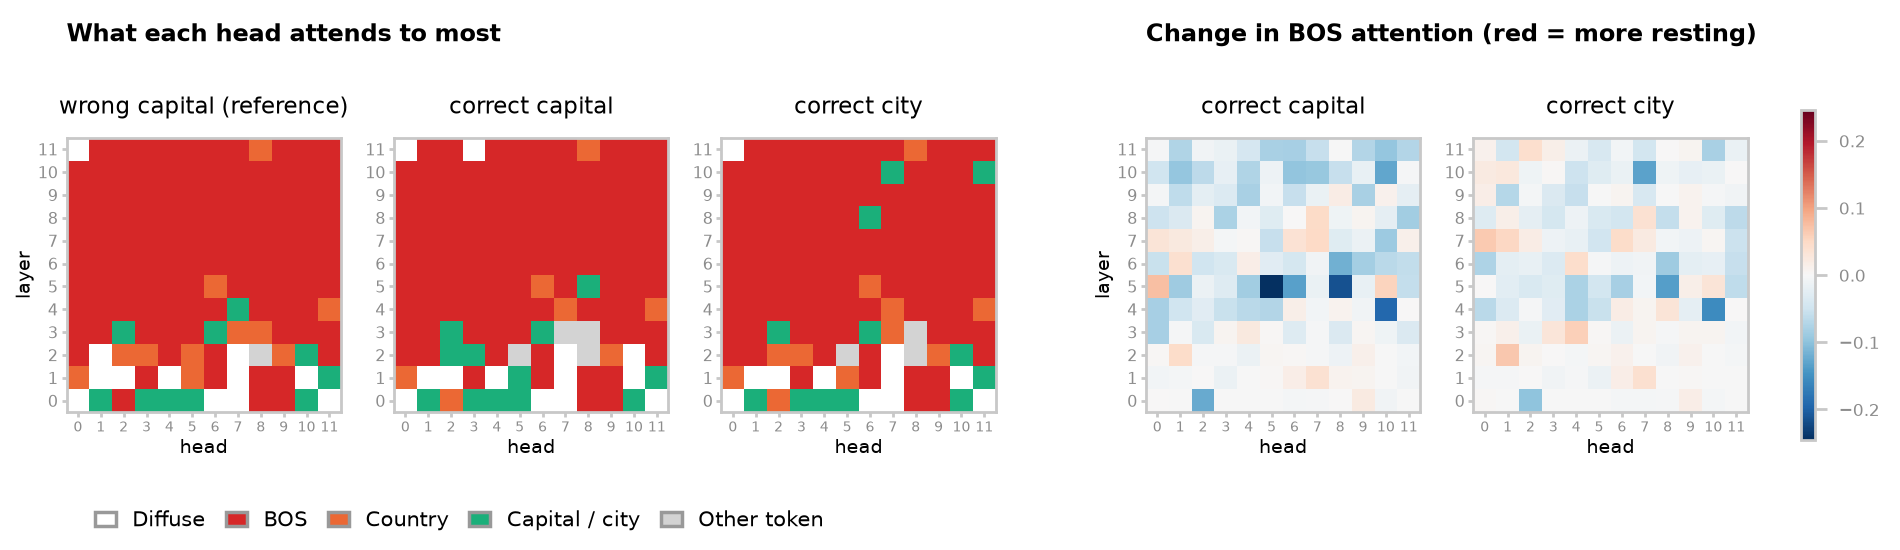
\includegraphics[width=\linewidth]{exp9_strip.png}\raggedright


\vspace{10pt}
%=========================== EXPERIMENT 10 ===========================
\head{Experiment 10 · the country anywhere earlier}{496 placements \,·\, 50 rows per filler type}

\vspace{2pt}
\centering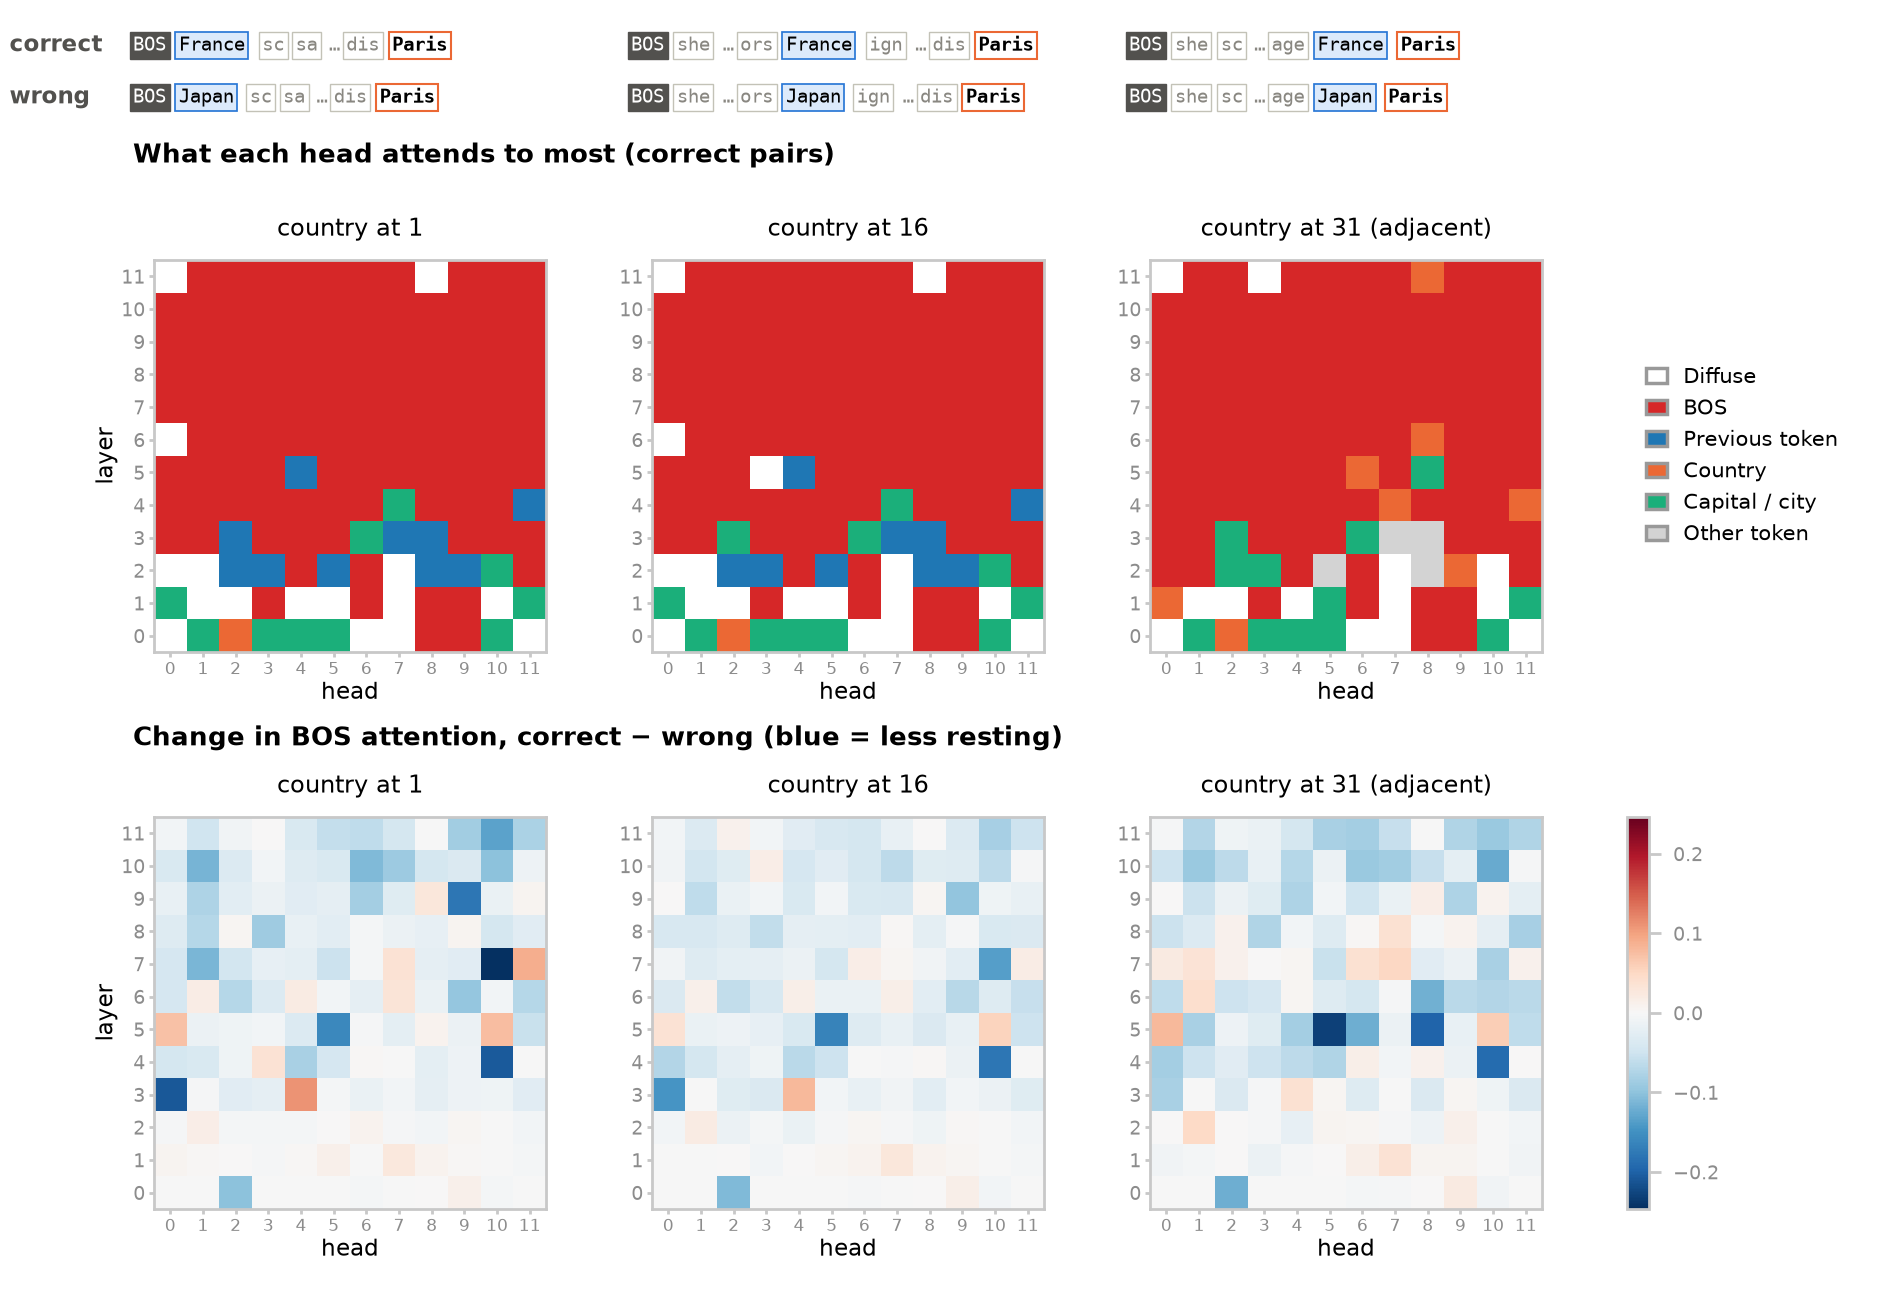
\includegraphics[width=\linewidth]{exp10_fig.png}\raggedright


\vspace{10pt}
%=========================== TAKEAWAY + NEXT ===========================
\end{document}
